In this chapter, I will derive results for the scalar field theory which includes an interaction term $\frac{\lambda}{4!}\phi^4$. Note that this is not a gauge theory, as its Langrangian density is symmetric under $\mathbb{Z}_2$, i.e. $\phi\rightarrow -\phi$, which is discrete in nature. Thus, Noether's theorem cannot be applied. The interaction term is a self interaction, not a gauge interaction.

\section{Path Integral Formulation}
The path integral formulation in QM and QFT generalizes the action principle of classical mechanics. To compute a quantum amplitude, it replaces the classical notion of a single, unique trajectory for a system with a sum, or functional integral, over an infinity of quantum-mechanically possible trajectories.\\

\noindent To develop the path integral for a scalar field theory, I will first derive the formulation for a quantum mechanical phase space and then extend it to fields. The path integral gives us the probability for point-to-point transition in the phase space.\\ 

\noindent The transition amplitude is given by $\langle q_f,t_f|q_i,t_i\rangle$. After dividing time into $n$ infinitesimally small slices of step size $\tau$, a complete set of eigenstates is inserted.

$$\langle q_f,t_f|q_i,t_i\rangle=\int dq_1\cdots\int dq_n\, \langle q_f,t_f|q_n,t_n\rangle\langle q_n,t_n|q_{n-1},t_{n-1}\rangle\cdots\langle q_1,t_1|q_i,t_i\rangle$$\\

\noindent To evaluate this, the below formulas are used.
$$\langle q_{j+1},t_{j+1}|q_j,t_j\rangle=\langle q_{j+1}|e^{-iH\tau}|q_j\rangle\approx\delta(q_{j+1}-q_j)-i\tau\langle q_{j+1}|H|q_j\rangle$$
$$\delta(q_{j+1}-q_j)=\frac{1}{2\pi}\int dp\, e^{ip(q_{j+1}-q_j)}$$
$$\left\langle q_{j+1}\middle|\frac{p^2}{2m}\middle|q_j\right\rangle=\frac{1}{2\pi}\int dp\, e^{ip(q_{j+1}-q_j)} \frac{p^2}{2m}$$
$$\langle q_{j+1}|V(q)|q_j\rangle=\frac{V(q_j)}{2\pi}\int dp\, e^{ip(q_{j+1}-q_j)}$$\\

\noindent Inserting these expressions in their respective places, 
$$\langle q_{j+1},t_{j+1}|q_j,t_j\rangle=\frac{1}{2\pi}\int dp_j\, e^{i[p(q_{j+1}-q_j)-H\tau)]}$$
\begin{align*}
    \begin{split}
        \implies\langle q_f,t_f|q_i,t_i\rangle&=\lim_{n\to\infty}\int\prod_{j=1}^{n}dq_j\int\prod_{j=1}^{n}\frac{dp_j}{2\pi}\, e^{i\sum_{j=1}^{n}[p(q_{j+1}-q_j)-H\tau)]}\\
        &=\int\frac{\mathcal{D}q_j\mathcal{D}p_j}{2\pi}\, e^{i\int dt\, (p\dot q-H)}\propto\int\mathcal{D}q_j\, e^{iS}
    \end{split}
\end{align*}

\noindent Thus, we can infer that the transition amplitude is not a single path, but rather a weighted average of the histories of configurations in the phase space, with weights proportional to the action. In field theory, $q_j$ is replaced by $\phi$.

\section{Generating Functional}
A source term, $\mathcal{L}_\text{source}=J\phi$ is added to the original Lagrangian density to model the effect of external sources on fields. $J$ vanishes both at spatial infinity (at all times) and everywhere in both the remote past and in the remote future. Thus for $t=-\infty$ and $t=\infty$, the fields are in their ground state $|0\rangle$.\\

\noindent The generating functional is defined as $Z[J]=\langle 0|0\rangle \propto\mathcal{D}\phi\,e^{iS[\phi]}$. This is equivalent to the partition function in statistical mechanics, and just like the partition function, we can derive a lot of physics from this single quantity. In the asymptotically long time limit, it is equal to the path integral.

$$\langle\phi(x)|T[\phi(x_1)\phi(x_2)]|\phi(x')\rangle=\mathcal{N}\int\mathcal{D}\phi\,\phi(x_1)\phi(x_2)e^{i\int d^dx\,(\mathcal{L}+J\phi)}$$

\noindent Here, T is the time ordering operator to ensure ealier times are to the right and later times are to the left. Taking the double functional derivative, we obtain the two-point correlation function, denoted by $G^{(2)}$, is also known as the Feynman propagator of the scalar field. It gives us a probabilistic measure of how the field propagates between two points, such that both initial and final states are stable ground states, and the field interacts with other fields in the way.

$$G^{(2)}(x_1-x_2)=\frac{1}{Z[0]}\left[\frac{\delta^2 Z[J]}{\delta J(x_1)\delta J(x_2)}\right]_{J=0}=i^2 \langle 0|T[\phi(x_1)\phi(x_2)]|0\rangle$$\\

\noindent Suppose we have a $D=d+1$ dimensional Minkowski spacetime. An analytic continuation can be made to an Euclidean manifold via a Wick rotation, $x_0\rightarrow ix_D$. The Euclidean Lagrangian density for a free field coupled to source $J$ is $\mathcal{L}_E=\frac{1}{2}(\nabla_\mu\phi)^2+\frac{1}{2}m^2\phi^2-J\phi$. For the generating functional, its integral needs to be calculated, wherein the first term can be rewritten as $-\int\phi(\nabla^2\phi)\,d^Dx$ by invoking the $D$-dimensional Gauss theorem.

$$\mathcal{L}_E=\frac{1}{2}\phi(-\nabla^2+m^2)\phi-J\phi$$
$$\phi=\bar\phi+\xi$$
$$\implies\mathcal{L}_E=\frac{1}{2}\bar\phi(-\nabla^2+m^2)\bar\phi-J\bar\phi+\frac{1}{2}\xi(-\nabla^2+m^2)\xi+\xi(-\nabla^2+m^2)\bar\phi-J\xi$$

\noindent We can decouple the source by requiring the shift $\bar\phi$ be such that terms linear in $\xi$ cancel out.

$$\bar\phi=(-\nabla^2+m^2)^{-1}J$$
$$\implies\bar\phi(x)=\int d^Dx'\,G_0^{(2)}(x-x')J(x')$$

\noindent The propagator, $G_0^{(2)}=\langle x|(-\nabla^2+m^2)^{-1}|x'\rangle$, is the Green's function for the field equation. The subscript 0 denotes free field.

$$Z[J]\propto e^{\frac{1}{2}\int d^Dx\,d^Dx'\,J(x)G_0^{(2)}(x-x')J(x')}$$

\noindent Now, I will take into account the effects of the $\phi^4$ interaction term by splitting the action into $S_0+S_\text{int}$.

\begin{align*}
    \begin{split}
        e^{-S_\text{int}[\phi]}&=e^{-\int d^Dx\,\frac{\lambda}{4!}\phi^4(x)}\\
        &=\sum_{n=0}^{\infty} \frac{-1^n}{n!}\left(\frac{\lambda}{4!}\right)^n \int d^Dx_1\cdots\int d^Dx_n\,\phi^4(x_1)\cdots\phi^4(x_n) 
    \end{split}
\end{align*}

\begin{align*}
    \begin{split}
        Z[J]&=\sum_{n=0}^{\infty} \frac{-1^n}{n!}\left(\frac{\lambda}{4!}\right)^n \int d^Dx_1\cdots\int d^Dx_n\,\frac{\delta^4}{\delta J^4(x_1)}\cdots \frac{\delta^4}{\delta J^4(x_n)}Z_0[J]\\
        &=e^{-\frac{\lambda}{4!}\int d^Dx\,\frac{\delta}{\delta J^4(x)}}Z_0[J]\\
        &=e^{-S_\text{int}\left[\frac{\delta}{\delta J}\right]} Z_0[J]
    \end{split}
\end{align*}

\section{Feynman Rules}
The Feynman rules calculate the contribution of an interaction between two fields at different coordinates via the interaction strength and the propagator. Since the generating functional with interactions contains an exponential term in $\lambda$, we need to model it by perturbative expansion and consider its effect at each order. I will construct the model upto first order in $\lambda$.\\

\noindent For zeroth order, $Z[J]=Z_0[J]$ and $G(x_1-x_2)=G_0(x_1-x_2)+\mathcal{O}(\lambda)$. For first order, however,

$$Z[J]=1-\frac{\lambda}{4!}\int dy\,\frac{\delta^4}{\delta J^4(y)}Z_0[J]$$\\

\noindent $Z_0[J]$ must be expanded upto atleast second order to get non-vanishing terms.

$$\int d^Dx\,\frac{\delta^4}{\delta J^4(x)}\frac{1}{2!}\left(\frac{1}{2}\int d^Dy_1\int d^Dy_2J(y_1)G_0(y_1-y_2)J(y_2)\right)^2$$

\noindent The derivatives yield a set of delta functions with 4! permutations.

$$Z[0]=1-\left(\frac{\lambda}{4!}\right)S\int dx\,(G_0(x-x))^2+\mathcal{O}(\lambda^2)$$

\noindent $S$ is the multiplicity factor, which counts all the ways in which the same Feynman diagram can be obtained by contracting lines in a pairwise fashion without changing the topology. Here, $S=3$. This diagram (vaccuum fluctuation) is given as

\begin{center}
    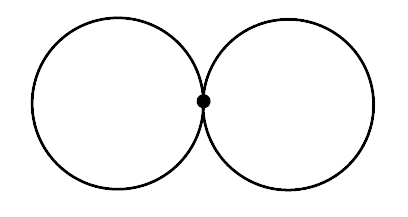
\includegraphics[scale=0.5]{vac_fluc}
\end{center}

\noindent Now, first order corrections to $\frac{\delta^2 Z[J]}{\delta J(x_1)\delta J(x_2)}$ can be obtained by expanding $Z_0[J]$ upto 3rd order.

$$\int d^Dy\,\frac{\delta^2}{\delta J^4(x_1)\delta J^4(x_2)}\frac{\delta^4}{\delta J^4(y)}\frac{1}{3!}\left(\frac{1}{2}\int d^Dz_1\int d^Dz_2J(z_1)G_0(z_1-z_2)J(z_2)\right)^3$$

\noindent which gives us six factors of source $J$ at $z_1\cdots z_6$, and six derivatives, one at $x_1$, one at $x_2$ and four at $y$. The non-vanishing Feynman diagrams are, 

\begin{center}
    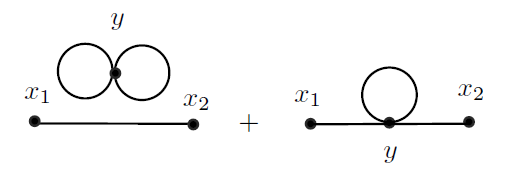
\includegraphics{green_1st}
\end{center}

\noindent The first term is $G_0(x_1-x_2)\left[\frac{-\lambda}{8}\int d^Dy\,(G_0(y-y))^2\right]$ and the second term is $\left(\frac{-\lambda}{8}\right)S\int d^Dy\,G_0(x_1-y)G_0(y-x_2)$. Here, $S=4\times 3\times 1=12$ (4 ways of contracting one external point to one of the lines attached to the vertex, 3 ways to do it for another point, 1 way to contract the two leftover lines to the vertex). Therefore, the full propagator becomes

\begin{center}
    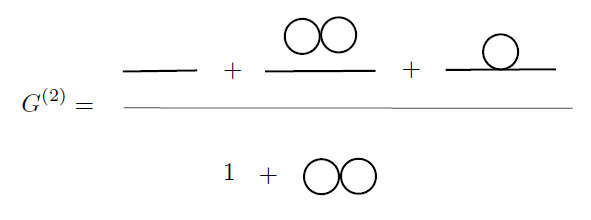
\includegraphics[scale=0.75]{cancel_1}
    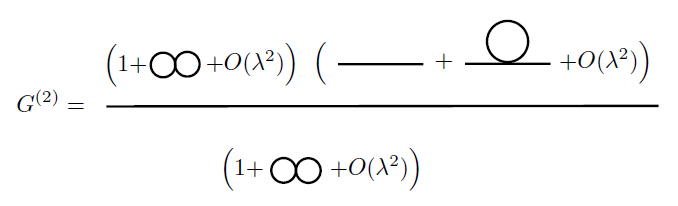
\includegraphics[scale=0.75]{cancel_2}
\end{center}

\noindent The vaccuum fluctuation cancels out. 

$$G^{(2)}(x_1-x_2)=G_0^{(2)}(x_1-x_2)-\frac{\lambda}{2}\int d^Dy\,G_0^{(2)}(x_1-y)G_0^{(2)}(y-x_2)+\mathcal{O}(\lambda^2)$$

\noindent Diagramatically, each vertex contributes $\lambda$ to the amplitude, and propagation between two internal points $z_1$ to $z_2$ is given by the correlation function. The result is then integrated over each internal point and internal loop.